\chapter{Application des méthodes au problème}

    Dans cette partie, nous allons présenter comment les diverses techniques que nous souhaitons appliquer sont compatibles avec notre cas spécifique du sudoku.
    \section{A*}
    \section{Algorithme génétique}
        Pour spécifier notre instance générale d'algorithme génétique, nous avons 4 éléments à définir
        \begin{itemize}
            \item Les génomes
            \item La sélection des meilleurs génomes
            \item Le croisement de différents génomes
            \item La mutation d'un génome
        \end{itemize}
        Pour certains de ces éléments, il peut exister différentes manières de procéder, nous allons donc en détailler plusieurs.
        \section{Génomes}
            Dans un premier temps, il nous faut nous poser la question de comment représenter notre grille de sudoku sous un format propice à un algorithme génétique.\\
            \subsection{Méthode 1D}
                Dans beaucoup de cas, travailler sur un tableau à une dimension simplifie énormément le travail. Nous allons donc procéder comme suit:
                \begin{description}
                    \item[Grille sudoku vide]:\\
                        \begin{center}
                            \begin{tabular}{|c|c|c| |c|c|c| |c|c|c|}
                                \hline
                                &\textbf{1}&&&&\textbf{3}&&&\\
                                \hline
                                &&&\textbf{4}&&&&&\\
                                \hline
                                &&&&\textbf{2}&&&&\\
                                \hline
                                \hline
                                &&&\textbf{7}&&&&&\\
                                \hline
                                \textbf{8}&&&&&&&\textbf{6}&\\
                                \hline
                                &&\textbf{5}&&&&&&\\
                                \hline
                                \hline
                                &&&&\textbf{3}&&&&\textbf{9}\\
                                \hline
                                &\textbf{3}&&&&&\textbf{1}&&\\
                                \hline
                                &&&&\textbf{6}&&&&\\
                                \hline
                            \end{tabular}
                        \end{center}
                    \item[G\'enome]: Un tableau d'une dimension contenant uniquement le contenu des cases \textbf{non données} dans l'énonce.
                \end{description}
            \subsection{Méthode 2D}
                Cependant il subsiste des cas où il est important de garder l'aspect 2D pour faciliter les traitements qui seront fait dessus par la suite.\\
                Dans ces cas ci, on garde un tableau 2D de ``cases'', qui seront une pair contenant une valeur, et si cette case est donnée dans l'énoncé
        \section{Sélection}
        \section{Croisement}
            Le croisement des génomes sélectionnés est la méthode la plus importante de tout l'algorithme, car c'est la méthodes qui sera en charge de ``passer'' les gains d'information précédents aux nouveaux génomes.\\
            Deux méthodes peuvent être employées:
            \begin{itemize}
                \item Croisement naïf
                \item Croisement optimisé
            \end{itemize}
            \subsection{Croisement naïf}
                Ce croisement utilise un génome basé sur le modèle 1D.\\
                Le but de ce dernier est de fonctionner rapidement, et à défaut d'être efficace rapidement, il utilise l'aléatoire pour favoriser un mélange hétéroclite sur plusieurs générations.\\
                \subsubsection{Fonctionnement}
                    Donnons nous 2 génomes tirés aléatoirement parmi ceux sélectionnés lors de la phase précédente.\\
                    \begin{description}
                        \item[Genome 1]:\\
                            \begin{tabular}{|c|c|c|c|c|c|c|c|c|c|}
                                \hline
                                g_1&g_1&g_1&g_1&g_1&g_1&g_1&g_1&g_1&g_1
                                \hline
                            \end{tabular}
                        \item[Genome 2]:\\
                    \end{description}
                \subsection{Croisement optimisé}
        \section{Mutation}


    \section{Eco-résolution}
    \subsection{Modélisation}
    Dans le chapitre, présentation des différents modèles nous avons présentés les divers attributs des eco-agents ainsi que leurs principales fonctions. \\
    L'éco-résolution est un mode de résolution utilisant plusieurs agents, la partie la plus complexe étant de définir quels sont nos agents et comment ils agissent entre eux. \\
    Nous avons ainsi défini le diagramme de classe suivant : \\
    \begin{center}
    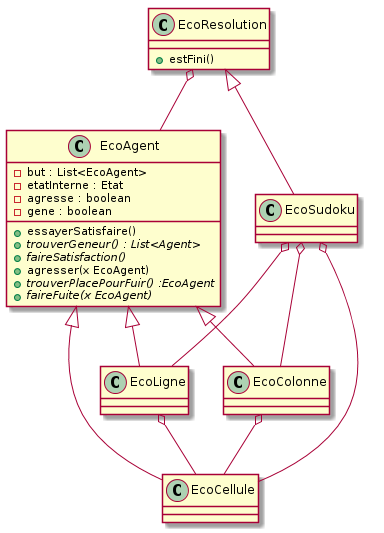
\includegraphics[scale=0.7]{diagrams/ecoResolution.png}
    \end{center} 

	Pour l'éco-résolution, nous retrouvons une seule méthode estFini(), qui vérifie lorsque tous les éco-agents de notre système sont satisfaits. \\
	Avant de démarrer l'éco-résolution, nous allons compléter les cases vides de notre sudoku. Les cases étant déjà dans l'énoncé comporteront un attribut cellType valant "GIVEN". Pour remplir notre sudoku, nous allons effectué un remplissage "intelligent", c'est-à-dire que dans chaque bloc nous allons placer une et une seule fois chaque numéro de 1 à 9.\\
	Nous avons choisi que nos cellules, nos lignes et nos colonnes seraient considérés comme éco-agent. \\
	
	\subsubsection{Les lignes}
	Nous allons voir les lignes comme éco-agent de la manière suivante : \\
	\begin{itemize}
	\item Le but d'une ligne est que tous les éco-agents qui la compose (cellule) aient des numéros différents.
	\item Pour trouver les gêneurs, cela correspondra à toutes les cellules qui ont un numéro qui intervient plus d'une fois. 
	\item FaireSatisfaction : Passer l'état comme étant satisfait
	\item une ligne ne pourra ni fuir, ni être en recherche de fuite.   
	\end{itemize}
	
	\subsubsection{Les colonnes}
	Nous allons voir les colonnes comme éco-agent de la manière suivante, analogue à la façon dont nous voyons les lignes : \\
	\begin{itemize}
	\item Le but d'une colonne est que tous les éco-agents qui la compose (cellule) aient des numéros différents.
	\item Pour trouver les gêneurs, cela correspondra à toutes les cellules qui ont un numéro qui intervient plus d'une fois. 
	\item FaireSatisfaction : Passer l'état comme étant satisfait
	\item une colonne ne pourra ni fuir, ni être en recherche de fuite.   
	\end{itemize}
	
	\subsubsection{Les cellules}
	Nous allons voir les cellules comme des agents de la manière suivante : 
	\begin{itemize}
	\item Une cellule est satisfaite si sa ligne et sa colonne sont satisfaites
	\item Les gêneurs d'une cellule sont les numéros ayant la même valeur sur la colonne et la ligne
	\item Pour FaireSatisfaction d'une cellule, il faut qu'il n'y ai plus de gêneur
	\item Pour trouverPlacePourFuir d'une cellule nous avons plusieurs idées : choisir une cellule aléatoirement dans le même bloc, choisir une cellule aléatoirement dans le bloc mais qui ne soit pas sur la ligne ou colonne de notre agent qui lance l'agression et enfin choisir la cellule qui a le plus de gêne.
	\item Pour faireFuite, nous allons échanger les numéros de nos deux cellules.
	\end{itemize}
	
	\subsection{Diagramme de séquence}
		\subsubsection{SeSatisfaire}
		\begin{center}
    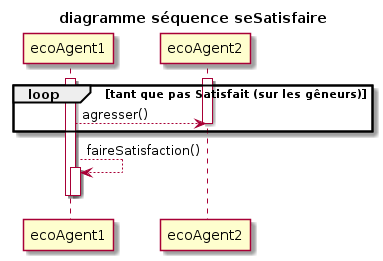
\includegraphics[scale=0.7]{diagrams/sequenceEcoResolution1.png}
    \end{center} 
    Pour se satisfaire un éco-agent agresse tous les autres agents qui le gênent. Une fois qu'il n'est plus gêné il est satisfait. 
		\subsubsection{Fuir}
\begin{center}
    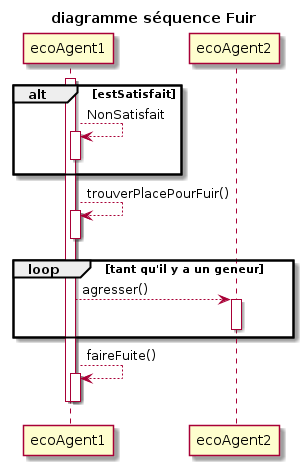
\includegraphics[scale=0.7]{diagrams/sequenceEcoResolution2.png}
    \end{center} 
    Si un agent doit fuir et qu'il est satisfait il devient non satisfait. Ensuite il recherche une place pour fuir, agresse tous les gêneurs qui l'empêche de fuir puis fait fuite. 